\documentclass{article}
\usepackage{tikz}
\usepackage[simplified]{pgf-umlcd}
\usetikzlibrary{arrows, arrows.meta}

\begin{document}

\title{
    Tarea 1 - Modelo y Diccionario \\
    INF239 - BASES DE DATOS
}
\author{
    Matias Peñaloza 202373037-8 \\
    Integrante2 Rol2
}
\date{
    2025-1
}
\maketitle

\section{Modelo}
\subsection{Entidad-Relación General}
Antes de realizar el modelo de la base de datos, analizaremos las entidades y relaciones presentes.

\begin{center}
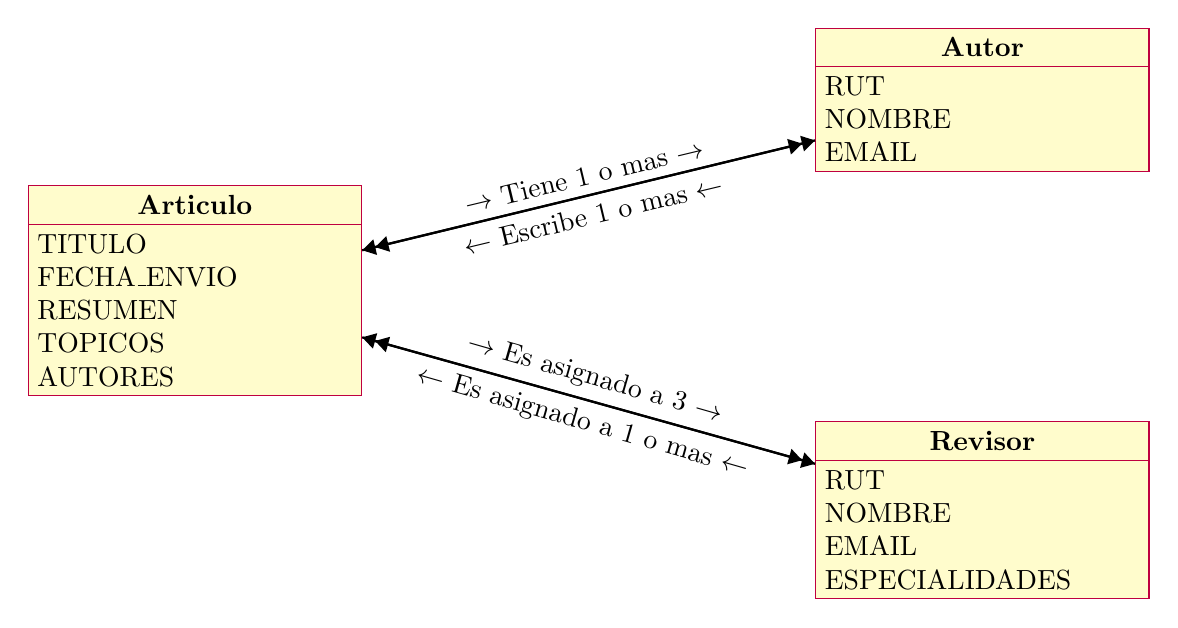
\begin{tikzpicture}
\begin{class}[text width=4cm]{Articulo}{0 ,-2}
    \attribute{TITULO}
    \attribute{FECHA\_ENVIO}
    \attribute{RESUMEN}
    \attribute{TOPICOS}
    \attribute{AUTORES}
\end{class}

\begin{class}[text width=4cm]{Autor}{10 ,0}
    \attribute{RUT}
    \attribute{NOMBRE}
    \attribute{EMAIL}
\end{class}

\begin{class}[text width=4cm]{Revisor}{10 ,-5}
    \attribute{RUT}
    \attribute{NOMBRE}
    \attribute{EMAIL}
    \attribute{ESPECIALIDADES}
\end{class}

\draw [thick,-{Triangle}{Triangle}] (Articulo) --++ (Revisor) node[midway, rotate=-16, above] {$\rightarrow$ Es asignado a 3 $\rightarrow$};
\draw [thick,-{Triangle}{Triangle}] (Revisor) --++ (Articulo) node[midway, rotate=-16, below] {$\leftarrow$ Es asignado a 1 o mas $\leftarrow$};

\draw [thick,-{Triangle}{Triangle}] (Articulo) --++ (Autor) node[midway, rotate=13.5, above] {$\rightarrow$ Tiene 1 o mas $\rightarrow$};
\draw [thick,-{Triangle}{Triangle}] (Autor) --++ (Articulo) node[midway, rotate=13.5, below] {$\leftarrow$ Escribe 1 o mas $\leftarrow$};

\end{tikzpicture}
\end{center}

\subsection{Modelo BD}
Ahora podemos llevar el modelo general de la situacion a un modelo de base de datos.

\begin{center}
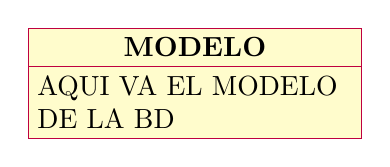
\begin{tikzpicture}
    \begin{class}[text width=4cm]{MODELO}{0 ,0}
        \attribute{AQUI VA EL MODELO DE LA BD}
    \end{class}
\end{tikzpicture}
\end{center}

\section{Diccionario de Datos}


\end{document}
